% !TeX root = slides_template.tex
% Insert inside the existing Beamer document, before its references frame.
% No document wrapper or additional packages are required by slides_template.tex.
% Image paths match the final Overleaf paper supplied by Benjamin.

% !TeX root = slides_template.tex

\begin{frame}{Motivation: Market Regimes}
\begin{itemize}
\item Market regimes describe distinct periods of return behavior, but the underlying states are \textbf{unobserved}.
\item Identifying these regimes may help characterize changing market conditions and inform investment decisions.
\item Common models for modeling financial returns such as Geometric Brownian Motion assumes constant drift and volatility, which limits its ability to represent these changes.
\item Therefore, unsupervised learning algorithms that explicitly model regime-switching is a suitable model for this type of problems.
\end{itemize}
\end{frame}

\begin{frame}{Hidden Markov Model}
\begin{itemize}
    \item Hidden Markov Model (HMM) is an unsupervised learning probabilistic model. 
    \item Assume that the sequences of observations (market data) $x_{1:T}$ are generated by latent states (regimes) $z_{1:T}$, where the latent states evolve according to a first-order Markov chain. \cite{rabiner1989}
    \item First-order Markov assumption (i.e. memoryless after 1 time lag)
    \item Assume observations conditionally independent given latent state
\end{itemize}

\end{frame}

\begin{frame}{HMM Training}
\begin{itemize}
    \item HMM is learns its parameter with Baum-Welch algorithm, a type of Expectation-Maximization algorithm for HMMs \cite{rabiner1989}.
    \item \textbf{E-step:} Use forward--backward to compute
    posterior probabilities of hidden states and transitions.

    \item \textbf{M-step:} Update initial probabilities,
    transition probabilities, and emission parameters using
    these posterior probabilities as weights.

    \item Repeat until the log-likelihood converges or the
    iteration limit is reached.
\end{itemize}

\[
\hat{\theta}
=
\arg\max_{\theta}
\log p_{\theta}(x_{1:T}),
\qquad
\theta=(\boldsymbol{\pi},A,\boldsymbol{\theta}_{\mathrm{emission}}).
\]
\end{frame}

\begin{frame}{Baum-Welch algorithm}
    \begin{figure}
        \centering
        \includegraphics[width=0.7\linewidth]{Midterm/artifacts/baum-welch.png}
        \label{fig:baum-welch}
    \end{figure}
\end{frame}

\begin{frame}{HMM Inference}
    \begin{itemize}
        \item Given a sequence of observations and fitted parameters, HMM returns the most probable hidden state sequence via the Viterbi algorithm \cite{rabiner1989}.
        \item Using dynamic programming to track the best path ending in each state, then backtrack to recover the overall best path.
    \end{itemize}
\end{frame}

\begin{frame}{Viterbi algorithm}
    \begin{figure}
        \centering
        \includegraphics[width=0.8\linewidth]{Midterm/artifacts/viterbi.png}
        \label{fig:viterbi}
    \end{figure}
\end{frame}

\begin{frame}{Graphical Representation of HMM}
\begin{figure}[ht]
    \centering

    \begin{tikzpicture}[
        scale=0.9,
        transform shape,
        node distance=2.5cm and 3.2cm,
        latent/.style={
            circle,
            draw,
            minimum size=1.4cm,
            font=\large
        },
        observed/.style={
            circle,
            draw,
            fill=gray!35,
            minimum size=1.4cm,
            font=\large
        },
        arrow/.style={
            -{Latex[length=3mm]},
            thick
        }
    ]

        % Hidden states
        \node[latent] (z1) {$z_1$};
        \node[latent, right=of z1] (z2) {$z_2$};
        \node[right=2.3cm of z2, font=\Large] (dots1) {$\cdots$};
        \node[latent, right=2.3cm of dots1] (zT) {$z_T$};

        % Observations
        \node[observed, below=1.7cm of z1] (x1) {$\mathbf{x}_1$};
        \node[observed, below=1.7cm of z2] (x2) {$\mathbf{x}_2$};
        \node[below=of dots1, font=\Large] (dots2) {$\cdots$};
        \node[observed, below=1.7cm of zT] (xT) {$\mathbf{x}_T$};

        % Transition arrows with probabilities
        \draw[arrow]
            (z1) -- node[above] {$p(z_2 \mid z_1)$} (z2);

        \draw[arrow]
            (z2) -- node[above] {$p(z_3 \mid z_2)$} (dots1);

        \draw[arrow]
            (dots1) -- node[above] {$p(z_T \mid z_{T-1})$} (zT);

        % Emission arrows with probabilities
        \draw[arrow]
            (z1) -- node[left] {$p(\mathbf{x}_1 \mid z_1)$} (x1);

        \draw[arrow]
            (z2) -- node[left] {$p(\mathbf{x}_2 \mid z_2)$} (x2);

        \draw[arrow]
            (zT) -- node[left] {$p(\mathbf{x}_T \mid z_T)$} (xT);

    \end{tikzpicture}

    \caption{Hidden Markov model as a directed graph.}
    \label{fig:hmm-probabilities}
\end{figure}
\end{frame}

\begin{frame}{Emission Models}
\begin{itemize}
    \item The emission distribution $p(x_t|z_t)$ models how each hidden regime gives rise to the observed features.
    \item Typically, Gaussian distribution is used, parameterized by mean $\mu$ and variance $\sigma^2$.
\end{itemize}

Problem:
\begin{itemize}
    \item Financial asset returns exhibit well-known stylized facts such as heavy tails, skewness, and volatility clustering \cite{rcont2001}.
    \item  The Gaussian assumption may be restrictive when the distribution of returns within a regime exhibit these characteristics on financial data.
\end{itemize}
\end{frame}

\begin{frame}{Research Questions}
This motivates us to look for more flexibility in the emission model. We consider the following research questions:
\begin{itemize}
    \item What's the consequence of using Gaussian emission model to represent data that is not Gaussian?
    \item Does a more flexible emission model improves the detection of regimes? Up until this midterm stage, we consider using Gaussian Mixture Models.
    \item Does the identified regimes provide useful information for investment decisions?
\end{itemize}
\end{frame}

\begin{frame}{Recent Research in Emission Representation}

\begin{itemize}
    \item \textbf{Heavy-tailed emissions:}
    Peruilh Bagolini et al. (2026) use multivariate Student-$t$
    emissions in a Bayesian HMM to model cryptocurrency returns \cite{bagolini2026}. 

    \item \textbf{Flexible parametric distributions:}
    Foroni et al. (2024) use state-dependent generalized
    hyperbolic distributions to model financial dependence
    networks \cite{foroni2024}.

    \item \textbf{Neural density models:}
    Lorek et al. (2022) introduce FlowHMM, using normalizing flows to learn each state's emission density \cite{lorek2022}.
\end{itemize}

\begin{alertblock}{Connection to our study}
Flexible emissions can better represent within-state dynamics. We will investigate how more flexible emissions improve regime detection over Gaussian, and the feasibility of neural density models like normalizing flow on financial time series data in the near future.
\end{alertblock}

\end{frame}

\begin{frame}{Gaussian vs. Gaussian mixture emissions}
\small
\begin{columns}[T,onlytextwidth]
\column{0.47\textwidth}
\textbf{Gaussian HMM}
\[
p_k(x)=\mathcal N(x;\mu_k,\sigma_k^2)
\]
\begin{itemize}
\item One Gaussian per state.
\item Simple mean and variance interpretation.
\item Restrictive for skewness and heavy tails.
\end{itemize}
\column{0.49\textwidth}
\textbf{Gaussian mixture HMM}
\[
p_k(x)=\sum_{m=1}^{M}w_{km}\mathcal N(x;\mu_{km},\sigma_{km}^2)
\]
\begin{itemize}
\item Multiple Gaussian components within each state.
\item Have greater flexiblility in describing the target distribution.
\item More parameters and greater fitting cost.
\end{itemize}
\end{columns}
\vspace{0.3cm}

\end{frame}

\begin{frame}{Challenges in Evaluation}
Evaluating regime-switching models on financial data in general remains an open challenge.

\textbf{Problems}:
    \begin{itemize}
        \item We won't be able to evaluate the model on its regime detection capabilities on real financial data because no true regime label exist.
        \item There is no one standard definition for market regime. Bull/bear markets and high/low volatility describe different aspects of market behavior and can all be considered the definition of different regimes.
        \item There is generally also no universally accepted standardized benchmarks for regime-switching models in finance. Differences in
    datasets, regime definitions, and evaluation protocols
    limit comparisons across studies \cite{davi2026}.
    \end{itemize}
These limitations motivate our use of complementary synthetic and real-data experiments.
\end{frame}

\begin{frame}{Evaluation Methodology}

\textbf{Synthetic data: controlled evaluation}
\begin{itemize}
    \item Known regime labels and generating distributions
    allow direct evaluation of state, emission, and
    transition recovery.

    \item Vary emission shape and regime persistence to
    examine when each model succeeds or fails.
\end{itemize}

\medskip

\textbf{Real data: practical evaluation}
\begin{itemize}
    \item Evaluate performance under market behavior that
    controlled simulations may not capture.

    \item Assess out-of-sample distributional fit and whether
    regime-based signals improve downstream trading
    performance.
\end{itemize}

\end{frame}

\begin{frame}{Synthetic experimental design}
\begin{columns}[T,onlytextwidth]
\column{0.48\textwidth}
\textbf{Generating families}
\begin{itemize}
\item Gaussian: correctly specified baseline.
\item Student-$t$: heavy tails.
\item Trimodal mixture: multimodality.
\item Shifted Gamma: skewness.
\end{itemize}
\column{0.48\textwidth}
\textbf{Common fitting protocol}
\begin{itemize}
\item 20,000 training; 5,000 test points.
\item 10 independent replications.
\item 10 starts; retain highest training likelihood.
\item At most 1,000 EM updates per start.
\end{itemize}
\end{columns}
\vspace{0.25cm}
\begin{itemize}
    \item Independent train and test sequences to test models' ability to generalize to another realization
    \item We do 10 different initializations in an attempt to get a better optima as Baum-Welch is sensitive to initialization \cite{rabiner1989}.
\end{itemize}
Identical observations for both models; independent train and test sequences.
Families are matched in state-specific means and variances within each setting.
\end{frame}

\begin{frame}{Two Types of Synthetic Regimes}
We define 2 types of synthetic regimes: First by emissions distribution in each state vary by their mean and hold their standard deviation fixed, and the other where we vary their stardard deviation and hold mean fixed.

\centering
\begin{tabular}{lcc}
\toprule
 & Mean-separated & Volatility-defined \\
\midrule
State means & $(-2,0,2)$ & $(0,0,0)$ \\
State standard deviations & $(1,1,1)$ & $(1,2,4)$ \\
Self-transition probability & $0.995$ & $0.995$ \\
\bottomrule
\end{tabular}\par
\[
A_{kk}=p,\qquad A_{kj}=(1-p)/2\ (j\ne k),\qquad \pi_k=1/3.
\]
\end{frame}

\begin{frame}{Synthetic Data Generation}
    \begin{enumerate}
    \item Sample the initial hidden state from a categorical distribution defined by the initial probabilities,
    \[
    z_1 \sim \mathrm{Categorical}(\boldsymbol{\pi}).
    \]

    \item For each subsequent time step, sample the hidden state according to the
    transition probabilities of the previous state,
    \[
    z_t \mid z_{t-1} \sim
    \mathrm{Categorical}\!\left(A_{z_{t-1}}\right).
    \]

    \item The sampled state $z_t$ determines the corresponding emission distribution.

    \item Sample the observation from that state-specific distribution,
    \[
    x_t \mid z_t=k \sim p_k(x).
    \]

    \item Repeat for $t=1,\ldots,T$ to obtain the hidden-state sequence
    $z_{1:T}$ and observation sequence $x_{1:T}$.
\end{enumerate}
\end{frame}

\begin{frame}{Example of Synthetic Data}
    \begin{figure}[H]
    \centering
    \includegraphics[width=0.75\linewidth]{Midterm/artifacts/synthetic-regime-example.png}
    \caption{An example of Student-$t$ based emission synthetic data partitioned by regimes}
    \label{fig:synthetic-regime-example}
\end{figure}
\end{frame}

\begin{frame}{Evaluation Metrics}
\begin{tabular}{p{0.28\linewidth}p{0.64\linewidth}}
\toprule
Measure & What it evaluates \\
\midrule
Macro F1 / accuracy & Agreement with known synthetic states \\
Emission KL divergence & Recovery of each state's generating density \\
Transition RMSE & Recovery of the generating transition matrix \\
Decoded switch count & How often the inferred state sequence changes \\
\bottomrule
\end{tabular}\par
\vspace{0.35cm}
\end{frame}

\begin{frame}{Problem: Arbitrary Labels}

\begin{itemize}
    \item HMM hidden-state labels are \alert{arbitrary}.
    \item The model is not told which state should be called 0, 1, or 2.
\end{itemize}

\vspace{0.4cm}

\begin{align*}
    \text{True states:} &
    \qquad
0 \quad 1 \quad 2 \\
\text{Learned states:} &
\qquad
2 \quad 0 \quad 1
\end{align*}

\vspace{0.3cm}

These can represent the \alert{same regimes}, only with different labels.

\[
\boxed{
\text{State labels must be aligned before evaluation}
}
\]

\end{frame}

\begin{frame}{Solution: Arbitrary Labels}
We use a similar approach to Wiedenhoeft et al. by solving a linear assignment problem that maximizes agreement between training Viterbi predictions and true training states \cite{wiedenhoeft2016}.
\begin{enumerate}
    \item Fit the HMM using only training observations.
    \item Use known synthetic training labels to find the state mapping which maximizes the total number of matched observations.
    \item Freeze this mapping.
    \item Apply it to predictions on the test set.
\end{enumerate}

\vspace{0.2cm}


\footnotesize
Solved using \texttt{scipy.optimize.linear\_sum\_assignment}.

\end{frame}

\begin{frame}{Mean-Separated Regimes: State and Density Recovery}
\small
\centering
\setlength{\tabcolsep}{5pt}
\begin{tabular}{llrrr}
\toprule
Family & Model & Macro F1
& Accuracy & Emission KL \\
\midrule
Gaussian & GHMM
& 0.9980 & 0.9980 & 0.00015 \\
& GMM-HMM
& 0.9979 & 0.9980 & 0.00038 \\
\addlinespace
Student-$t$ & GHMM
& 0.9901 & 0.9907 & 0.49280 \\
& GMM-HMM
& \textbf{0.9991} & \textbf{0.9992} & \textbf{0.01046} \\
\addlinespace
Trimodal & GHMM
& 0.9975 & 0.9976 & 0.29469 \\
& GMM-HMM
& \textbf{0.9984} & \textbf{0.9985} & \textbf{0.00051} \\
\addlinespace
Skewed Gamma & GHMM
& 0.9971 & 0.9973 & 0.08905 \\
& GMM-HMM
& \textbf{0.9984} & \textbf{0.9985} & \textbf{0.00679} \\
\bottomrule
\end{tabular}\par

\vspace{0.2cm}
\begin{itemize}
    \item Both models achieve high state-classification performance.
    \item GMM-HMM substantially improves non-Gaussian density fit.
    \item Accurate state recovery can coexist with emission misspecification.
\end{itemize}
\end{frame}

\begin{frame}{Mean-Separated Regimes: Fitted Densities Graph}
    \begin{figure}[H]
    \centering
    \includegraphics[width=0.6\linewidth]{Midterm/artifacts/mean-regime-densities.jpg}
    \caption{An example of fitted densities from GHMM and GMM-HMM overlayed on the true generating densities for mean-separated regimes in a replicate}
    \label{fig:mean-regime-densities}
\end{figure}
\end{frame}

\begin{frame}{Volatility-Defined Regimes: State and Density Recovery}
\small
\centering
\setlength{\tabcolsep}{5pt}
\begin{tabular}{llrrr}
\toprule
Family & Model & Macro F1
& Accuracy & Emission KL \\
\midrule
Gaussian & GHMM
& 0.9806 & 0.9813 & 0.00017 \\
& GMM-HMM
& 0.9806 & 0.9812 & 0.00044 \\
\addlinespace
Student-$t$ & GHMM
& 0.4855 & 0.5675 & 1.01907 \\
& GMM-HMM
& \textbf{0.9527} & \textbf{0.9535} & \textbf{0.01061} \\
\addlinespace
Trimodal & GHMM
& 0.7003 & 0.7484 & 4.00752 \\
& GMM-HMM
& \textbf{0.9938} & \textbf{0.9941} & \textbf{0.00064} \\
\addlinespace
Skewed Gamma & GHMM
& 0.8415 & 0.8708 & 0.18228 \\
& GMM-HMM
& \textbf{0.9837} & \textbf{0.9842} & \textbf{0.00685} \\
\bottomrule
\end{tabular}\par

\vspace{0.2cm}
\begin{itemize}
    \item Comparable classification under Gaussian emissions.
    \item GMM-HMM improves state recovery across non-Gaussian families.
    \item Lower emission KL accompanies substantially stronger classification.
\end{itemize}

\end{frame}

\begin{frame}{Volatility-Defined Regimes: Fitted Densities Graph}
    \begin{figure}
        \centering
        \IfFileExists{Midterm/artifacts/volatility-densities-plot.png}{%
            \includegraphics[width=0.6\linewidth]{Midterm/artifacts/volatility-densities-plot.png}%
        }{%
            \IfFileExists{image/midterm_report_scratch/volatility-densities-plot.png}{%
                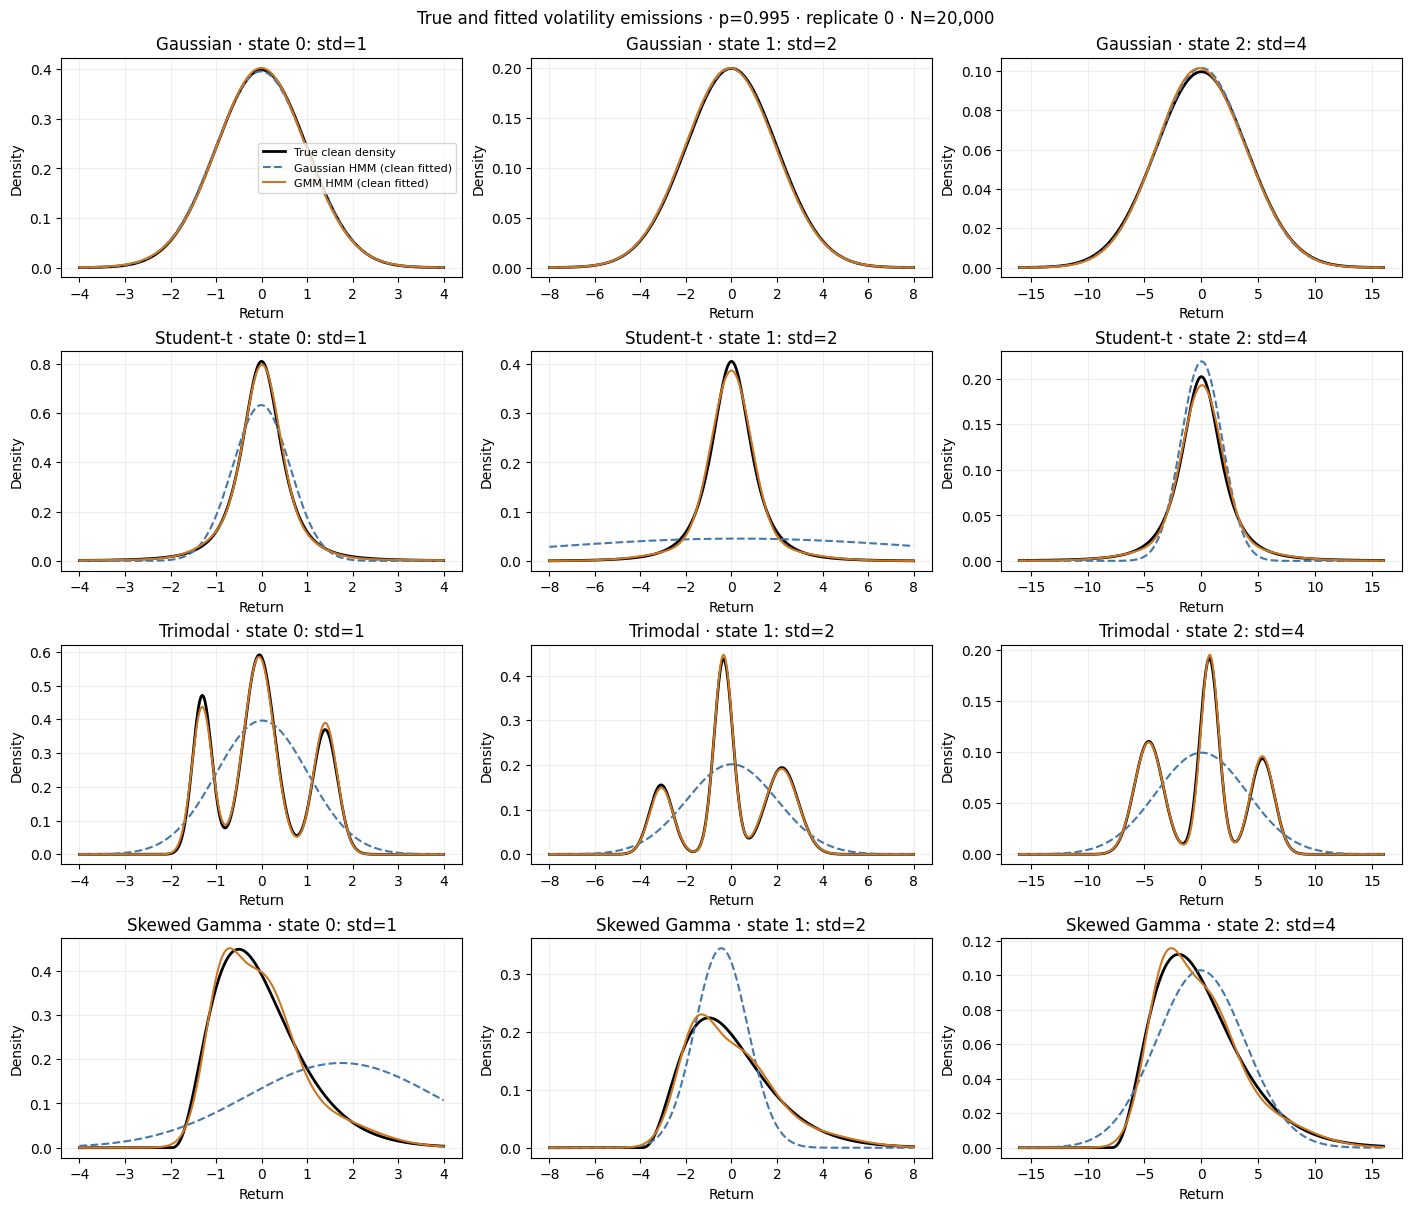
\includegraphics[width=0.6\linewidth]{image/midterm_report_scratch/volatility-densities-plot.png}%
            }{%
                \fbox{\parbox{0.8\linewidth}{\centering
                    Figure not available locally.\\[6pt]
                    Upload \texttt{volatility-densities-plot.png} to\\
                    \texttt{Midterm/artifacts/} to display this plot.}}%
            }%
        }
        \label{fig:volatility-densities-plot}
    \end{figure}
\end{frame}

\begin{frame}{Mean-Separated Regimes: Transition Recovery and Switching}
\small
\centering
\setlength{\tabcolsep}{7pt}
\begin{tabular}{lrrrr}
\toprule
& \multicolumn{2}{c}{Transition RMSE}
& \multicolumn{2}{c}{Average decoded switches} \\
Family & GHMM & GMM-HMM & GHMM & GMM-HMM \\
\midrule
Gaussian     & 0.00088 & 0.00087 & 24.4 & 24.4 \\
Student-$t$  & 0.01075 & \textbf{0.00088} & 73.6 & 24.7 \\
Trimodal     & 0.00083 & 0.00086 & 24.1 & 24.2 \\
Skewed Gamma & 0.00167 & \textbf{0.00088} & 28.6 & 24.4 \\
\bottomrule
\end{tabular}\par

\vspace{0.3cm}
\alert{True average: 23.8 switches per test sequence.}

\begin{itemize}
    \item Both models closely recover transitions under
    Gaussian, trimodal, and skewed Gamma emissions.
    \item GHMM over-switches under Student-$t$ emissions,
    despite its high classification accuracy.
\end{itemize}
\end{frame}


\begin{frame}{Volatility-Defined Regimes: Transition Recovery and Switching}
\small
\centering
\setlength{\tabcolsep}{7pt}
\begin{tabular}{lrrrr}
\toprule
& \multicolumn{2}{c}{Transition RMSE}
& \multicolumn{2}{c}{Average decoded switches} \\
Family & GHMM & GMM-HMM & GHMM & GMM-HMM \\
\midrule
Gaussian     & 0.00071 & 0.00069 & 26.0  & 26.1 \\
Student-$t$  & 0.40839 & \textbf{0.00092} & 486.4 & 23.7 \\
Trimodal     & 0.25389 & \textbf{0.00070} & 542.1 & 28.4 \\
Skewed Gamma & 0.10875 & \textbf{0.00081} & 170.6 & 26.8 \\
\bottomrule
\end{tabular}\par

\vspace{0.3cm}
\alert{True average: 28.8 switches per test sequence.}

\begin{itemize}
    \item GHMM substantially over-switches and incorrectly estimates transitions under non-Gaussian emissions.
    \item GMM-HMM estimates transitions accurately and produces
    switch counts close to the truth.
\end{itemize}
\end{frame}

\begin{frame}{Example of GHMM Over-Switching}
  \begin{figure}[H]
    \centering
    \includegraphics[width=0.7\linewidth]{Midterm/artifacts/decoded-regimes-student-t.png}
    \label{fig:decoded-regimes-student-t}
\end{figure}  
\end{frame}

\begin{frame}{Interpreting GHMM's performance degration on volatility regimes}

\begin{itemize}
    \item Mean-separated regimes provide location differences
    that help distinguish states despite emission misspecification.

    \item Volatility-defined regimes share the same mean.
    identifying them depends more on correctly representing
    distributional spread and tails. 
    
    \item GMM-HMM remained robust to this while GHMM started to mix up regimes, causing rapid switching and inaccurate classification.

    \item Moreover, GHMM performed the worst on Student-$t$ (heavy-tailed) data while GMM-HMM remained robust.
\end{itemize}

\begin{alertblock}{Examining the fitted state structure}
Do the inferred states represent generating regimes,
or different parts of their emission distributions?
\end{alertblock}

\end{frame}


\begin{frame}{Selected failures for Student-$t$: a state used for extreme observations}
\small
\textbf{Two mean-separated Student-$t$ replications}
\begin{center}
\begin{tabular}{lrr}
\toprule
GHMM diagnostic & Replication 5 & Replication 8 \\
\midrule
Test extreme observations captured & 61.2\% & 56.5\% \\
\bottomrule
\end{tabular}\par
\end{center}
\begin{itemize}
\item A broad, low-persistence fitted state captures extreme observations.
\item Another fitted state receives over 98\% of training observations from \emph{each} of two true regimes.
\item Extremes satisfy $|x_t-\mu_{z_t}|/\sigma_{z_t}>3$, using generating-state moments.
\end{itemize}
\alert{Consistent with states representing tail variation while true regimes merge.}
\end{frame}

\begin{frame}{Selected failures for Student-$t$: a state used for extreme observations}
    \begin{figure}[H]
    \centering
    \includegraphics[width=0.75\linewidth]{Midterm/artifacts/cm-student-t.png}
    \caption{Confusion matrix of true versus aligned fitted state for GHMM and GMM-HMM on a replicate of Student-$t$ emission data}
    \label{fig:confusion-matrix-student-t}
\end{figure}
\end{frame}

\begin{frame}{Interpreting GHMM and GMM-HMM's performance on volatility and Student-$t$}
    \begin{itemize}
        \item Gaussian emission was too restrictive for this case. GHMM wrongly merged majority of the observations in the tails of all states into one state trying to explain the variation of the model, while merging most of the observations in two true states into one regime.
        \item GMM-HMM was able to distinguish this through the use of its three components in each state and assigned most of tail observations to one component and the center observations to the other 2 components while preserving state structure. (i.e. mixture components can represent central and tail observations within a state)
        \item These cases illustrate how flexible emissions can capture within-regime variation while preserving the distinction between regimes, supporting more accurate state recovery.
    \end{itemize}
\end{frame}

\begin{frame}{Excessive Switching: Is it a problem?}
    \begin{itemize}
        \item Usually, it signifies model overfitting to the noise
        \item Classification accuracy can hide this problem, brief incorrect excursions affect few observations but introduce multiple false transitions.
        \item In real-world financial applications, if regime changes trigger portfolio adjustments, false switches may increase turnover and transaction costs.
        \item This is highlighted by Shu et al. \cite{shu2024regime}, who compared HMM-based strategy against JM-based (Jump Model) strategy, and hightlighted that JM achieved better risk-adjusted return metrics due to its lower tendency for excessive switching.
    \end{itemize}
\end{frame}

\begin{frame}{Conclusion on Synthetic Experiment}

    \begin{itemize}
    \item GMM-HMM better approximates the non-Gaussian generating distributions, with comparable classification under Gaussian emissions.

    \item Both models recover persistent mean-separated states accurately, while GMM-HMM achieves substantially better recovery of non-Gaussian volatility regimes.

    \item GMM-HMM produces regimes that contains a lot less excessive switching and closer to the true switch counts compared to GHMM.

    \item High accuracy can coexist with excessive switching, inaccurate transitions, and poor emission-density fit.
\end{itemize}

Flexible emissions can improve regime recovery by representing
complex variation within states, but improved synthetic results
do not establish real-market usefulness.
\end{frame}

\begin{frame}{S\&P 500: Experimental Setup}
\begin{itemize}
    \item Compare Gaussian, Student-$t$, and GMM emissions with $M=2$ or $3$.
    \item Two hidden states, interpreted as relatively bullish and bearish conditions.
    \item Evaluate on 5,534 decision dates from 2004 to 2025.
    \item Start with ten years of training history, then expand the sample.
    \item Refit the scaler, PCA, and HMM every 63 decisions and use up to three EM updates between refits.
\end{itemize}
\end{frame}

\begin{frame}{From Prices to Trading Positions}
\begin{itemize}
    \item Calculate daily simple returns, rolling downside deviation, and Sortino-style features.
    \item Use 5, 10, and 60-day rolling windows and EWMA half-lives.
    \item Standardize 28 features and apply PCA, retaining at least 95\% of the variance.
    \item Forecast next-day bull probability with the HMM.
    \item Using 12-decision rolling median of raw bull threshold above 50\%
    \item Hold the index when bullish, otherwise hold cash.
\end{itemize}
\source{Feature construction: \cite{shu2024regime,king2025bulls}. PCA: \cite{jolliffe2016pca}.}
\end{frame}

\begin{frame}{Rolling Downside Deviation}
\small
Daily simple return and target-relative return:
\[
 r_t=\frac{P_t}{P_{t-1}}-1,
 \qquad x_t=r_t-\tau,\qquad \tau=0.
\]
Clip nonnegative returns to zero: $z_t=\min(x_t,0)$.
\[
 \bar z_{t,n}=\frac{1}{n}\sum_{j=0}^{n-1}z_{t-j},
 \qquad
 D_{t,n}=\sqrt{\frac{1}{n}\sum_{j=0}^{n-1}
 (z_{t-j}-\bar z_{t,n})^2}.
\]
\begin{itemize}
    \item Use trailing windows $n\in\{5,10,60\}$ trading days.
    \item Calculate the population standard deviation of the clipped returns, including the zeros.
\end{itemize}
\end{frame}

\begin{frame}{Sortino-Style Features}
The trailing mean target-relative return is divided by downside deviation:
\[
 S_{t,n}=\frac{\displaystyle\frac{1}{n}\sum_{j=0}^{n-1}x_{t-j}}
 {\max(D_{t,n},10^{-6})},
 \qquad n\in\{5,10,60\}.
\]
\begin{itemize}
    \item The denominator floor prevents division by zero.
    \item Also calculate EWMAs of returns, downside deviation, and Sortino-style features with 5, 10, and 60-day half-lives.
    \item Use only current and past observations, and drop incomplete warm-up rows before fitting.
\end{itemize}
\source{Related feature construction: \cite{shu2024regime,king2025bulls}.}
\end{frame}

\begin{frame}{Baseline Strategies}
\begin{itemize}
    \item \textbf{Buy-and-hold:} Stay fully invested in the S\&P 500 throughout the evaluation period.
    \item \textbf{MA 50/200:} Hold the index when its trailing 50-day average price exceeds its trailing 200-day average; otherwise hold cash.
\end{itemize}
\[
 \overline P_{t,n}=\frac{1}{n}\sum_{j=0}^{n-1}P_{t-j},
 \qquad
 w_t^{\mathrm{MA}}=\mathbf{1}\{\overline P_{t,50}>\overline P_{t,200}\}.
\]
\begin{itemize}
    \item Positions use information available through day $t$ and earn the next day's return $R_{t+1}^{\mathrm{strategy}}=w_t r_{t+1}$.
    \item Both baselines use the same evaluation dates as the HMM strategies. Cash earns zero; dividends and trading costs are excluded.
\end{itemize}
\end{frame}

\begin{frame}{HMM Strategies: State Labels and Forecasts}
\begin{itemize}
    \item Compare Gaussian, Student-$t$, and GMM ($M=2,3$) emissions using the same features and trading rule.
    \item Label the state with the higher probability-weighted mean training return as \textbf{bull}; label the other state \textbf{bear}.
    \item Filter observations through day $t$ to obtain $\alpha_{t,k}=P(z_t=k\mid x_{1:t})$.
    \item Use the transition matrix to forecast the next day's bull probability:
\end{itemize}
\[
 q_t=P(z_{t+1}=\mathrm{bull}\mid x_{1:t})
     =\sum_{k=1}^{2}\alpha_{t,k}A_{k,\mathrm{bull}},
 \qquad b_t=\mathbf{1}\{q_t\geq 0.5\}.
\]
\small The trading forecast uses filtering, not a Viterbi path decoded using future observations.
\end{frame}

\begin{frame}{HMM Strategies: From Forecasts to Positions}
\begin{itemize}
    \item Smooth the binary forecasts $b_t$ using a trailing 12-decision rolling median $m_t$.
    \item Hold the index when the median is above $0.5$; hold cash when it is below $0.5$. A tie preserves the previous position.
\end{itemize}
\[
 w_t=
 \begin{cases}
  1, & m_t>0.5,\\
  0, & m_t<0.5,\\
  w_{t-1}, & m_t=0.5.
 \end{cases}
 \qquad R_{t+1}^{\mathrm{HMM}}=w_t r_{t+1}.
\]
\begin{itemize}
    \item Use available decisions during the initial 12-decision warm-up and initialize the previous position to cash.
    \item Long-only, fully invested or cash, and no short selling or leverage
\end{itemize}
\end{frame}

\begin{frame}{Strategy Growth: 2004--2025}
\centering
\includegraphics[width=\linewidth,height=0.65\textheight,keepaspectratio]{Midterm/artifacts/sp500/2004_2025_performance.png}
\par\medskip
\small Buy-and-hold has the highest total return. Risk-adjusted performance differs.
\end{frame}

\begin{frame}{Strategy Performance: 2004--2025}
\centering
\small
\begin{tabular}{@{}lrrr@{}}
\toprule
Strategy & Total return (\%) & Sharpe & Max.\ drawdown (\%) \\
\midrule
Student-$t$ & 251.7 & \textbf{0.640} & $-21.4$ \\
GMM ($M=3$) & 379.6 & 0.544 & $-33.9$ \\
MA 50/200 & 332.9 & 0.494 & $-33.9$ \\
Buy-and-hold & \textbf{517.6} & 0.439 & $-56.8$ \\
GMM ($M=2$) & 138.6 & 0.356 & $-29.2$ \\
Gaussian & 60.6 & 0.243 & $-23.9$ \\
\bottomrule
\end{tabular}
\par\medskip
\begin{itemize}
    \item Student-$t$ and GMM ($M=3$) have higher Sharpe ratios than both baselines.
    \item Returns exclude dividends, cash interest, and trading costs.
\end{itemize}
\end{frame}

\begin{frame}{Do the Forecasts Separate Market Conditions?}
\centering
\small
\begin{tabular}{@{}lrr@{}}
\toprule
Model & Bull: next-day return (\%) & Bear: next-day return (\%) \\
\midrule
GMM ($M=2$) & 0.0343 & 0.0433 \\
GMM ($M=3$) & 0.0581 & 0.0171 \\
Gaussian & 0.0441 & 0.0388 \\
Student-$t$ & 0.0550 & 0.0274 \\
\bottomrule
\end{tabular}
\par\medskip
\begin{itemize}
    \item GMM ($M=3$) and Student-$t$ give clearer return separation.
    \item Their smoothed positions last 55.9 and 49.9 trading days on average, including both invested and cash periods.
    \item Persistent signals and higher returns do not establish regime accuracy: true market-state labels are unavailable.
\end{itemize}
\end{frame}

\begin{frame}{Case Study: Signals During 2008}
\centering
\begin{figure}
    \includegraphics[width=\linewidth,height=0.79\textheight,keepaspectratio]{Midterm/artifacts/sp500/2008_strategy_replay.png}
    \caption{Blue and yellow lines indicate the $b_t$ and 12-decision rolling median $m_t$ ($m_t = 1$ means all-in S\&P 500)}
\end{figure}
\end{frame}

\begin{frame}{2008 Emission Densities: Gaussian}
\centering
\includegraphics[width=\linewidth,height=0.68\textheight,keepaspectratio]{Midterm/artifacts/sp500/2008_gaussian_density.png}
\par\medskip
\small September 2 and December 31, 2008: bull- and bear-state marginal densities of the standardized return feature.
\end{frame}

\begin{frame}{2008 Emission Densities: Student-t}
\centering
\includegraphics[width=\linewidth,height=0.68\textheight,keepaspectratio]{Midterm/artifacts/sp500/2008_studentt_density.png}
\par\medskip
\small September 2 and December 31, 2008: bull- and bear-state marginal densities of the standardized return feature.
\end{frame}

\begin{frame}{2008 Emission Densities: GMM ($M=2$)}
\centering
\includegraphics[width=\linewidth,height=0.68\textheight,keepaspectratio]{Midterm/artifacts/sp500/2008_gmm2_density.png}
\par\medskip
\small September 2 and December 31, 2008: bull- and bear-state marginal densities of the standardized return feature.
\end{frame}

\begin{frame}{2008 Emission Densities: GMM ($M=3$)}
\centering
\includegraphics[width=\linewidth,height=0.68\textheight,keepaspectratio]{Midterm/artifacts/sp500/2008_gmm3_density.png}
\par\medskip
\small September 2 and December 31, 2008: bull- and bear-state marginal densities of the standardized return feature.
\end{frame}

\begin{frame}{Changing the Number of GMM Components}
\begin{itemize}
    \item Compare $M=2,3,4,5$ components per state between 2004 and 2013
    \item Start with five years of training history and keep the same refit and signal-smoothing rules.
    \item All models still have two hidden states. More mixture components do not mean more market regimes.
    \item Examine both trading performance and the fitted component densities.
\end{itemize}
\end{frame}

\begin{frame}{GMM Component Sweep: Strategy Growth}
\centering
\includegraphics[width=\linewidth,height=0.65\textheight,keepaspectratio]{Midterm/artifacts/sp500/gmm_component_sweep.png}
\par\medskip
\small Three components give the strongest GMM strategy in this sweep, but MA 50/200 still performs better.
\end{frame}

\begin{frame}{GMM Component Sweep: Results}
\centering
\small
\begin{tabular}{@{}lrrrr@{}}
\toprule
Strategy & Return (\%) & Sharpe & Switches/year & Days/position \\
\midrule
GMM ($M=2$) & 53.0 & 0.277 & 5.41 & 45.76 \\
GMM ($M=3$) & 84.2 & 0.507 & 5.41 & 45.76 \\
GMM ($M=4$) & 17.9 & 0.110 & 4.61 & 53.55 \\
GMM ($M=5$) & 22.7 & 0.191 & 4.91 & 50.34 \\
MA 50/200   & 91.7 & 0.541 & 1.00 & 228.82 \\
Buy-and-hold & 65.3 & 0.246 & 0.00 & -- \\
\bottomrule
\end{tabular}
\par\medskip
\begin{itemize}
    \item More components do not improve trading performance here.
    \item The four- and five-component models switch less often after smoothing, so their weaker results are not simply caused by more frequent trading.
\end{itemize}
\end{frame}

\begin{frame}{Fitted GMM Densities Along PC1}
\centering
\includegraphics[width=\linewidth,height=0.79\textheight,keepaspectratio]{Midterm/artifacts/sp500/gmm_components_density.png}
\end{frame}

\begin{frame}{Component Locations and Mixture Weights}
\centering
\begin{figure}
    \includegraphics[width=\linewidth,height=0.76\textheight,keepaspectratio]{Midterm/artifacts/sp500/gmm_components_density_interval.png}
    \caption{The weight of each component in GMM is denoted by the number in the interval, and intervals are drawn by plus minus one standard deviation of the mean of PC1}
\end{figure}
\end{frame}

\begin{frame}{What Do the Components Represent?}
\begin{itemize}
    \item With two or three components, one component carries most of the bull-state weight. Smaller components describe variation around it or in the tails.
    \item With four or five components, more components overlap around the center, with small bull-state tail weights of roughly 0.04--0.07.
    \item These describe variation within the states, not separate market regimes.
    \item PC1 is not the market return. This projection alone cannot show whether the extra components fit useful structure or noise.
    \item The held-out-test is an experiment to explain the overfitting issue of GMM, but it's not included in this presentation.
\end{itemize}
\end{frame}

\begin{frame}{S\&P 500: Main Findings}
\begin{itemize}
    \item Student-$t$ and the three-component GMM improve risk-adjusted strategy performance relative to Gaussian emissions in the full-period experiment.
    \item The three-component GMM gives the strongest GMM strategy in the shorter sweep. Adding more components does not help here.
\end{itemize}
\end{frame}


\begin{frame}{Future Work: Normalizing Flow Emissions}
\begin{itemize}
    \item In the next few weeks, we'll focus on researching normalizing flows and its integration into HMM as an emission model. 
    \item Normalizing flows are deep-learning generative models that
transform a simple probability distribution into a more flexible distribution through a sequence of
invertible transformations \cite{papamakarios2021}.
    \item Rather than restricting each state’s emission density to a single Gaussian or a fixed finite Gaussian mixture, we will learn an invertible transformation of a base
distribution for each state. The resulting densities can be evaluated through the change-of-variables
formula and used within HMM inference.
    \item Given the limited observation amounts and the low signal-to-noise ratio of financial return data \cite{gu2020}, we’ll most likely need to investigate ways to prevent the NF-based emission model from overfitting to the noise.
\end{itemize}
\end{frame}

% Appendix and references are supplied by slides_template.tex.
% Keep this file insertable with \input in another presentation.
